\documentclass[11pt, oneside]{article}   	% use "amsart" instead of "article" for AMSLaTeX format
\usepackage[margin = 1in]{geometry}                		% See geometry.pdf to learn the layout options. There are lots.
\geometry{letterpaper}                   		% ... or a4paper or a5paper or ... 
%\geometry{landscape}                		% Activate for rotated page geometry
%\usepackage[parfill]{parskip}    		% Activate to begin paragraphs with an empty line rather than an indent
\usepackage{graphicx}				% Use pdf, png, jpg, or eps§ with pdflatex; use eps in DVI mode
								% TeX will automatically convert eps --> pdf in pdflatex		
\usepackage{amssymb}
\usepackage{amsmath}
\usepackage[shortlabels]{enumitem}
\usepackage{float}
\usepackage{tikz-cd}
\usepackage{subcaption}

\usepackage{amsthm}
\theoremstyle{definition}
\newtheorem{definition}{Definition}[section]
\newtheorem{theorem}{Theorem}[section]
\newtheorem{corollary}{Corollary}[theorem]
\newtheorem{lemma}[theorem]{Lemma}

\newcommand{\N}{\mathbb{N}}
\newcommand{\R}{\mathbb{R}}
\newcommand{\Z}{\mathbb{Z}}
\newcommand{\Q}{\mathbb{Q}}

\usepackage{simpler-wick}
\usepackage[compat=1.0.0]{tikz-feynman}   %note you need to compile this in LuaLaTeX for diagrams to render correctly

% make arrow superscripts
\DeclareFontFamily{OMS}{oasy}{\skewchar\font48 }
\DeclareFontShape{OMS}{oasy}{m}{n}{%
         <-5.5> oasy5     <5.5-6.5> oasy6
      <6.5-7.5> oasy7     <7.5-8.5> oasy8
      <8.5-9.5> oasy9     <9.5->  oasy10
      }{}
\DeclareFontShape{OMS}{oasy}{b}{n}{%
       <-6> oabsy5
      <6-8> oabsy7
      <8->  oabsy10
      }{}
\DeclareSymbolFont{oasy}{OMS}{oasy}{m}{n}
\SetSymbolFont{oasy}{bold}{OMS}{oasy}{b}{n}

\DeclareMathSymbol{\smallleftarrow}     {\mathrel}{oasy}{"20}
\DeclareMathSymbol{\smallrightarrow}    {\mathrel}{oasy}{"21}
\DeclareMathSymbol{\smallleftrightarrow}{\mathrel}{oasy}{"24}
%\newcommand{\cev}[1]{\reflectbox{\ensuremath{\vec{\reflectbox{\ensuremath{#1}}}}}}
\newcommand{\vecc}[1]{\overset{\scriptscriptstyle\smallrightarrow}{#1}}
\newcommand{\cev}[1]{\overset{\scriptscriptstyle\smallleftarrow}{#1}}
\newcommand{\cevvec}[1]{\overset{\scriptscriptstyle\smallleftrightarrow}{#1}}

\newcommand{\dbar}{d\hspace*{-0.08em}\bar{}\hspace*{0.1em}}

%SetFonts

%SetFonts


\title{8.325 Final Project: Local Operator Renormalization}
\author{Patrick Oare}
\date{}							% Activate to display a given date or no date

% If questions about the subject, talk to Iain.

\begin{document}

\maketitle

\thispagestyle{empty}

\section*{Abstract}

This paper will introduce local operator renormalization in the context of a general QFT and show how to renormalize 
such an operator perturbatively. We will show that operators in a QFT run with scale much like couplings, and develop 
a renormalization group equation for their Green's functions. Using an explicit example from the $\phi^3$ theory, 
we will see that renormalized operators mix under a scale transformation. We will conclude by examining non-perturbative features of local operator 
renormalization on the lattice, and show that the discrete nature of a lattice gauge theory leads to an interesting environment 
to study operator mixing. 

\newpage
\setcounter{page}{1}

\section{Introduction}

% Include motivation for why we want to do this. Maybe do a recap of basic renormalization stuff.
The primary purpose of renormalization in Quantum Field Theory is that of taming divergences. Given a Lagrangian, one 
can compute Green's functions in the theory and use the process of renormalization to render these observable results 
finite. This begs the question: what kind of Green's functions can we renormalize? Typically there is a focus on $n$-point 
functions of fields and operators at different points in spacetime, for example a correlator like $\langle 0 | 
T\{\phi_1(x_1) ... \phi_n(x_n)\} | 0\rangle$, which can be computed with standard techniques in perturbation theory. 

However, $n$-point correlation functions-- while very important in processes like scattering-- do not tell the whole story. 
We can also consider a \textbf{local composite operator}, which is an operator $\mathcal O(x)$ built up from the fields 
and derivatives in a theory at a single spacetime point $x$. Schematically for a theory with fermion fields $\{\Psi_i(x)\}$ 
and a gauge field $A_\mu$, such an operator looks like:
\begin{equation}
	\mathcal O_{\mu...\nu ... }(x) = D_{\mu}... A_{\nu}(x) ... \Gamma_{\ell_1} ... \Psi_{i_1}(x) ... 
	\overline \Psi_{j_1}(x) ...
\end{equation}
where the fields in this equation are the \textbf{renormalized fields} of the theory, obtained by renormalizing the 
$n$-point functions. One such example of a local composite operator is the QED current $j^\mu(x) = \overline\psi (x)
\gamma^\mu \psi(x)$, as it involves a product of fields at the same point. 
%Operators like this are particularly important in areas like lattice field theory, where one is able to directly compute Green's functions. 

% Discuss the OPE reasonably thoroughly (like in Collins ch 6.1)
Naively, because $\mathcal O(x)$ is composed of renormalized fields, one could think all its Green's functions will be 
finite. Unfortunately, this picture does not hold because of a subtlety which arises from the operator product expansion 
(OPE). Recall that the OPE allows us to expand a product of operators as a sum of other operators. For simplicity, we 
will assume we are working with renormalized scalar operators $\{\phi_i\}_{i}$, so that the OPE acts as:
\begin{equation}
	\phi_i(x)\phi_j(y) = \sum_k C_{ijk}(r, \partial_r) \phi_k(y)
\end{equation}
with $r = |x - y|$. The coefficients $C_{ijk}$ go as:
\begin{equation}
	C_{ijk}(r, \partial_r) = r^{\Delta_k - \Delta_i - \Delta_j}\left(1 + c r^\mu \partial_\mu + ...\right)
\end{equation}
As we take $x\rightarrow y$ to form a local composite operator, we take $r\rightarrow 0$, and because $C_{ijk}\sim 
r^{\Delta k - \Delta_i - \Delta_j}$, these coefficients $C_{ijk}$ will diverge. Thus if we compute a Green's function of 
a composite operator of renormalized fields, \textbf{we should expect additional divergences which are separate from 
the divergences of each individual field}. For example, the Green's function 
$\langle \phi(x)\phi(y)\rangle$ is rendered finite by renormalizing the operator $\phi$. However, because of the 
additional divergence in the OPE, there is no reason to assume that the Green's function $\langle\phi^2(x)\rangle$ 
will be finite, even when using the renormalized fields $\phi$. Therefore, we must develop a formalism to renormalize 
Green's functions of these local composite operators. 

For notation, we will use $|0\rangle$ to denote the vacuum, and $\langle ... \rangle$ to denote the time ordered 
correlator $\langle 0 | T\{...\} | 0\rangle$. 

\section{Theory}

% Recall how the renormalization process works?
To renormalize the fields and parameters involved in the computation of an $n$-point function, one computes the 
function with renormalized parameters, adds in the counterterm diagrams, then sets the sum to be finite. The 
counterterms are then picked to absorb the divergences, plus a finite scheme-dependent constant. We will follow a 
similar procedure to renormalize a local operator.

Suppose we wish to renormalize a local operator $\mathcal O(x)$ which is a product of the renormalized fields. The 
general procedure to renormalize this operator is to compute any non-vanishing Green's function involving 
$\mathcal O(x)$, and then renormalize this Green's function to render it finite. Typically, this will be of the form:
\begin{equation}
	\langle \mathcal O(x) \phi_{i_1}(x_1) ... \phi_{i_n}(x_n)\rangle
\end{equation}
along with some combination of derivatives. The $\phi_{i_k}$ label the possible fields that can be a part of the Green's 
function. Performing this procedure for one Green's function will render it finite for all other Green's functions. This is 
the same idea as in standard renormalization where once a field has been renormalized by computing a single 
Green's function containing it, all its other Green's functions will be finite (assuming every other operator in the Green's 
function is also renormalized). 

Before we can perform this renormalization, we must first discuss how to compute Green's functions perturbatively. As in 
the Feynman diagram expansion for $n$-point correlation functions, we split the Lagrangian into a free piece and an 
interaction piece $\mathcal L = \mathcal L_0 + \mathcal L_{int}$,where $\mathcal L_0$ describes a free field theory. We 
can compute a Green's function using the path integral approach:
\begin{align}
	\langle \mathcal O(x) \phi_{i_1}(x_1) ... \phi_{i_n}(x_n)\rangle &= \frac{1}{\mathcal Z} \int D\phi_i e^{i\int d^dz\,
	\mathcal L} \mathcal O(x) \phi_{i_1}(x_1) ... \phi_{i_n}(x_n) \\
	&= \frac{1}{\mathcal Z} \int D\phi_i e^{i\int d^d z \mathcal L_0} \sum_{k = 0}^\infty \frac{i^k}{k!}\left(\int \mathcal L_{int}
	\right)^k \mathcal O(x) \phi_{i_1}(x_1) ... \phi_{i_n}(x_n)
\end{align}
This equation looks almost exactly like the perturbative expansion for the $n$-point function, except there is an extra insertion of the operator $\mathcal O(x)$. This 
means that the diagrams we can draw to compute this Green's function will have the same Feynman rules as in the original theory, except we will have an 
additional vertex for the operator insertion, and each graph must contain exactly one operator insertion. 

These operator insertions act similar to standard Feynman rules, but they include a few novel features. In each diagram:
\begin{enumerate}
	\item Propagators are left attached to external legs. 
	\item Operators carry a momentum $q_\mu$ and can inject this momentum into their vertex.
	\item Certain operators can insert an additional structure into the calculation.
\end{enumerate}

As an example of this, we will consider a scalar field theory with a $\phi^3$ interaction given by:
\begin{equation}
	\mathcal L = \frac{1}{2}(\partial_\mu\phi)^2 - \frac{1}{2}m^2\phi^2 + \frac{g}{3!}\phi^3~
	\label{eq:phi_cubed}
\end{equation} 
We will return to this theory later when we study mixing. We shall consider the operator $\mathcal O(x) = \frac{1}{2}\phi^2(x)$. 
The $\frac{1}{2}$ is conventional, and is only there to pick up the symmetry factor of 2 associated with the tree level 
diagram. For this theory, the Feynman rules are the typical $\phi^3$ rules with an additional vertex denoting operator 
insertion. Because this operator is made of 2 composite fields, it will inject momentum into 2 legs. We can compute 
its correlation function with two fields at tree level by following out prescription:
\begin{equation}
\begin{gathered}
\langle \mathcal O(q) \phi(p_1) \phi(-p_2)\rangle = \feynmandiagram [large, horizontal'=a to c, baseline=(current bounding box.center)] {
a [particle = \(p_1\)] -- [insertion = {[size = 6pt, style = red] .5}] c [particle = \(p_2\)]
%a [particle = \(q_1\)] -- [fermion] b [dot, style = red],
%b -- [fermion] c [particle = \(q_2\)]
}; = \frac{i}{p_1^2 - m^2}\frac{i}{p_2^2 - m^2}
\end{gathered}~
\label{eq:tree}
\end{equation}
where the cross denotes an operator insertion. Notice that the value of this diagram is proportional to each propagator. 
Furthermore, momentum conservation implies that the injected momentum $q$ equals $p_2 - p_1$; $q$ can generally 
be nonzero. In this example, the operator injects no nontrivial structure into the amplitude since it is very simple. 

In the next section we will compute the one-loop correction to this Green's function. However, before we explore mixing 
in this theory we must finish our general discussion. Now that we have Feynman rules, we can in theory compute each 
Green's function we need. Let $\mathcal O^{(0)}$ be a local operator\footnote{$\mathcal O^{(0)}$ is still a composite 
object made of renormalized fields, even though we denote it as a bare object. We will call it the bare operator because 
it requires additional renormalization, as discussed in the first section.}. We define a renormalized operator:
\begin{equation}
	\mathcal O_R(\mu) := \mathcal Z_\mathcal{O} \mathcal O^{(0)}~
	\label{eq:renorm_op}
\end{equation}
and as usual, we split $\mathcal Z_\mathcal{O} = 1 + \delta_\mathcal{O}$. We will use the counterterm to absorb the 
divergence. Note that later when we introduce mixing, Equation~\ref{eq:renorm_op} will generalize to include more 
operators. However, that adds additional complexity for now, so we will only deal with operators in this section that do 
not mix. The counterterm has an associated diagram:
\begin{equation}
\begin{gathered}
\feynmandiagram [layered layout, horizontal=a to c, baseline=(current bounding box.center)] {
a [particle = \(p_1\)] -- b [crossed dot, style = red] -- c [particle = \(p_2\)]
%a [particle = \(q_1\)] -- [fermion] b [dot, style = red],
%b -- [fermion] c [particle = \(q_2\)]
}; = \frac{i}{p_1^2 - m^2}\delta_\mathcal{O}\frac{i}{p_2^2 - m^2}
\end{gathered}~
\label{eq:counter}
\end{equation}

Once the counterterm is determined, one can compute the \textbf{anomalous dimension} of the operator $\mathcal O$. 
This quantity plays the role of the $\beta$ function for operators, and describes how the operator flows under a change 
of scale. The anomalous dimension $\gamma_\mathcal{O}$ is formally defined to satisfy the following equation:
\begin{equation}
	\mu\frac{d}{d\mu}\mathcal O_R(\mu) = \gamma_\mathcal{O} \mathcal O_R(\mu)~
	\label{eq:anomalous}
\end{equation}

We are now in position to evaluate how the Green's function:
\begin{equation}
	G_n(x, x_1, ..., x_n) := \langle 0 | T\{\mathcal O(x) \phi(x_1) ... \phi(x_n)\} | 0\rangle
\end{equation}
flows under scale change. One can differentiate this and use the product rule to show that:
\begin{equation}
	\left[ \mu \frac{d}{d\mu} + \beta(g) \frac{d}{dg} + \frac{1}{2} n\gamma_\phi + \gamma_\mathcal{O} \right] G_n = 0
\end{equation}
This relation is known as the \textbf{Callan Symanzik equation}, and is an important relation between how the various 
couplings and fields flow under the renormalization group. Note that each term corresponds to an RG evolution of a 
specific part of the Green's function: the $\beta$ function for the coupling, the anomalous dimension $\gamma_\phi$ 
for the fields, and $\gamma_\mathcal{O}$ for the running of the operator. 

\section{Mixing}

When we renormalize a local operator, we typically need to be more general than Equation~\ref{eq:renorm_op} and 
include other bare operators in our expression for the renormalized operator. The divergences associated with 
Green's functions computed with the bare operator can generally have some structure which cannot be absorbed 
solely by a counterterm insertion for the original operator, hence we need more counterterm insertions to soak 
up the extra singularities. This phenomenon is called \textbf{operator mixing}. We will show by explicit example how this 
occurs in the $\phi^3$ theory, then take this story to the lattice, which offers a rich setting to study operator mixing. 

Suppose we wish to renormalize an operator $\mathcal O$ in our theory. Let $\{\Phi_i\}_{i\in I}$ be the set of all 
operators with mass dimensions $[\Phi_i] \leq \mathcal O$ which transform in the same way under all symmetries 
of the theory ($\Phi_i$ and $\mathcal O$ have the same \textbf{quantum numbers}). Then the renormalized 
$\mathcal O_R(\mu)$ can be written as a linear combination of all the $\{\Phi_i\}$:
\begin{equation}
	\mathcal O_R(\mu) = \sum_i \mathcal Z_{\mathcal{O}i} \Phi_i^{(0)}
\end{equation}
as opposed to simply saying that $\mathcal O_R = \mathcal Z_\mathcal{O} \mathcal O^{(0)}$. The renormalization 
coefficient is now promoted to a matrix in this space of operators $\mathcal Z_{ij}$, and the anomalous dimension 
likewise becomes a matrix $\gamma_{ij}$, and Equation~\ref{eq:anomalous} becomes:
\begin{equation}
	\mu\frac{d}{d\mu} \Phi_i^R(\mu) = \gamma_{ij} \Phi_j^{(0)}(\mu)
\end{equation}
This matrix differential equation can be solved to determine how the operator flows.

\subsection{$\phi^3$ theory}

To illustrate where mixing occurs, we will follow Collins~\cite{collins} and work with the $\phi^3$ theory 
given in Equation~\ref{eq:phi_cubed}. We renormalize the operator:
\begin{equation}
	\mathcal O(q) = \frac{1}{2}\phi^2(q)
\end{equation}

We have computed the tree level amplitude in Equation~\ref{eq:tree}, and the counterterm vertex in Equation~\ref{eq:counter}. 
There are four graphs that come in at one loop. 

\begin{figure}[H]
	\centering
	\begin{subfigure}[t]{.48\textwidth}
	\centering
	\feynmandiagram[layered layout, horizontal=b to c] {
		a -- [insertion = {[size = 6pt, style = red] .5}] b
		  -- [half left] c
		  -- [half left] b,
		c --  d
	};
	\caption*{(A)}
	\end{subfigure}
	~
	\begin{subfigure}[t]{.48\textwidth}
	\centering
	\feynmandiagram[layered layout, horizontal=b to c] {
		a -- b
		  -- [half left] c
		  -- [half left] b,
		c -- [insertion = {[size = 6pt, style = red] .5}] d
	};
	\caption*{(B)}
	\end{subfigure}
\\
	\begin{subfigure}[t]{.48\textwidth}
	\centering
	\vspace{.5cm}
	\feynmandiagram[layered layout, horizontal=b to c] {
		a -- [momentum = \(p_1\)] b
		  -- [half left, insertion = {[size = 6pt, style = red] .5}] c
		  -- [half left, momentum = \(k\)] b,
		c -- [momentum = \(p_2\)] d
	};
	\caption*{(C)}
	\end{subfigure}
	~
	\begin{subfigure}[t]{.48\textwidth}
	\centering
	\vspace{.5cm}
	%\feynmandiagram[layered layout, horizontal=a to c] {
		%a -- b -- d -- [half left, insertion = {[size = 6pt, style = red] .5}] e -- [half left] d,
	%	a -- b -- c,
	%	a -- b -- d -- [out = 45, in = -45, loop] d
	%};
	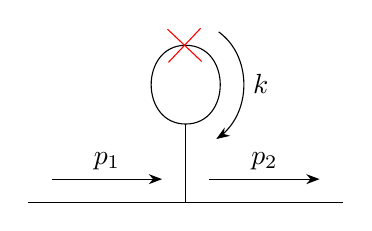
\begin{tikzpicture}
            \begin{feynman}
            \coordinate (a);
            \coordinate[left=2cm of a] (c);
            \coordinate[right=2cm of a] (b);
            \coordinate[above=1cm of a] (d);
            \coordinate[above=1cm of d] (e);
            \diagram* {
            %(b) -- [momentum = \(p_1\)] (a) -- [momentum = \(p_2\)] (c),
            (c) -- [momentum = \(p_1\)] (a) -- [momentum = \(p_2\)] (b),
            (a) -- (d) -- [half left, insertion = {[size = 6pt, style = red] .99}] (e)  -- [half left, momentum = \(k\)] (d)
            };
            \end{feynman}
            \end{tikzpicture}
	\caption*{(D)}
	\end{subfigure}
\end{figure}

The first two are already finite because the wavefunction renormalization $\delta_\phi$ renders the pure scalar loops 
finite. The third diagram is simple to compute in dimensional regularization, and using $d = 4 - \epsilon$ yields:
%\begin{equation}
%	\feynmandiagram[layered layout, horizontal=b to c] { a -- [insertion = {[size = 6pt, style = red] .5}] b -- c [crossed dot, label = \(\delta_\phi\)] 
%	--  d };  
%\end{equation}
%\begin{equation}
%	\feynmandiagram[layered layout, horizontal=b to c] {
%		a -- b [crossed dot, label = \(\delta_\phi\)]  -- d -- [insertion = {[size = 6pt, style = red] .5}] c
%	};
%\end{equation}
%render the $\phi$ loops finite. 
\begin{equation}
	(C) = \frac{g^2}{2(4\pi)^3} \frac{i}{p_1^2 - m^2}\frac{i}{p_2^2 - m^2} \left(\frac{2}{\epsilon} + \log(4\pi e^{-\gamma} 
	\mu^2)\right) + ...
\end{equation}
Note the divergent piece is proportional to the two propagators in the tree level Green's function, and thus this 
divergence can be picked up a counterterm from an $\mathcal O^{(0)}$ insertion. However, the second piece is a 
bit more complicated. The diagram equals:
\begin{equation}
	(D) = \frac{ig^2}{2(4\pi)^3} \frac{i}{p_1^2 - m^2} \frac{i}{p_2^2 - m^2} \frac{i}{(p_1 - p_2)^2 - m^2} 
	\left[m^2 - \frac{1}{6}(p_1 - p_2)^2\right] \left(\frac{2}{\epsilon} + \log(4\pi\mu^2 e^{\gamma - 1})\right) + ...~
	\label{eq:tadpole_div}
\end{equation}
Counterterms cannot depend on momentum, so this divergence \textbf{cannot} be picked up if we naively define 
out renormalized operator to be $\mathcal O_R = (1 + \delta_\mathcal{O})\mathcal O^{(0)}$. Instead, we need an 
operator which at tree level has this same momentum structure. From looking at the structure of the graph, it is clear that 
the operator that generates the tree level diagram:
\begin{equation}
	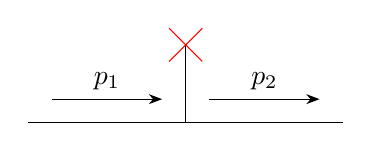
\begin{tikzpicture}[baseline=(current bounding box.center)]
            \begin{feynman}
            \coordinate (a);
            \coordinate[left=2cm of a] (c);
            \coordinate[right=2cm of a] (b);
            \coordinate[above=1cm of a] (d);
            \diagram* {
            %(b) -- [momentum = \(p_1\)] (a) -- [momentum = \(p_2\)] (c),
            (c) -- [momentum = \(p_1\)] (a) -- [momentum = \(p_2\)] (b),
            (a) -- [insertion = {[size = 6pt, style = red] .99}] (d)
            };
            \end{feynman}
            \end{tikzpicture} =  \frac{i}{p_1^2 - m^2} \frac{i}{p_2^2 - m^2} \frac{i}{(p_1 - p_2)^2 - m^2} (ig)
	\left[m^2 - \frac{1}{6}(p_1 - p_2)^2\right]
\end{equation}
will be able to absorb this divergence, as a corresponding counterterm insertion from this operator will be able to pick up 
the divergent piece attached to the propagator structure in Equation~\ref{eq:tadpole_div}. This graph is the tree level 
result for the correlator $\langle \Omega(q) \phi(p_1)\phi(-p_2)\rangle$, where $\Omega$ is the operator:
\begin{equation}
	\Omega := \left(m^2 + \frac{1}{6}\partial^2\right) \phi
\end{equation}

It is thus evident how to proceed: our prescription of $\mathcal O_R = \mathcal Z_\mathcal{O} \mathcal O^{(0)}$ is no 
longer sufficient to absorb every divergence. Instead, we define our renormalized operator by:
\begin{equation}
	\mathcal O_R := \mathcal Z_\mathcal{O} \mathcal O^{(0)} + \mathcal Z_\Omega \Omega^{(0)}
\end{equation}
where $\mathcal Z_\mathcal{O} = 1 + \delta_\mathcal{O} + ... $ and $\mathcal Z_\Omega = 0 + \delta_\Omega + ...$, 
since $\mathcal O_R$ must equal $\mathcal O^{(0)}$ at first order. We can read off the counterterms in MS:
\begin{equation}
	\delta_\mathcal{O} = -\frac{g^2}{(4\pi)^3}\frac{1}{\epsilon} \;\;\;\;\;\;\;\;\;\;\;\;\;\;\;\;\;\;\;\;\;\;\;\;\;\;\;\;\;\;
	\delta_\Omega = -\frac{g}{(4\pi)^3}\frac{1}{\epsilon}
\end{equation}
Using these counterterms, we see that the mixing matrix in the space spanned by $\{\frac{1}{2}\phi^2, \phi, 
\partial^2\phi\}$ is: 
\begin{equation}
	\begin{pmatrix} (\frac{1}{2}\phi^2)_R \\ \phi_R \\ (\partial^2\phi)_R \end{pmatrix} = 
	\begin{pmatrix} 1 + \delta_\mathcal{O} & m^2 \delta_\Omega & \frac{m^2}{6}\delta_\Omega \\ 
	0 & 1 + \delta_\phi & 0 \\ 0 & 0 & 1 + \delta_\phi \end{pmatrix}
	\begin{pmatrix} (\frac{1}{2}\phi^2)^{(0)} \\ \phi^{(0)} \\ \partial^2\phi^{(0)} \end{pmatrix}
\end{equation}
Note that the latter two operators are already renormalized through the renormalization of $\phi(x)$, since they do not 
suffer divergences in the OPE from being a local product. 

Although we showed this with a simple example from a scalar field theory, the moral of the story holds for any QFT. 
Whenever operators have the same quantum numbers, they are capable of mixing into one another. In practice, 
operators typically do not transform exactly identically and thus in most cases one can renormalize an operator 
without considering other structures it may mix into. However, there are certain situations where mixing is more frequent. 
One of these is that of lattice gauge theory, which we will now explore. 

\subsection{Mixing on the lattice}

The lattice is a playground for studying operator mixing because of its decreased symmetry relative to the continuum. 
When spacetime is discretized and a QFT is put on a (hypercubic) lattice, the symmetry group of our theory is 
reduced from $O(4)$ in the Euclidean continuum to $H(4)$, the group of symmetries of the hypercube. Because 
the lattice has significantly less symmetry than the continuum, it is easier for two operators to transform in the 
same way under the entire hypercubic group. To quantify this precisely, we need to classify how these symmetries 
act on operators in a theory: namely, we need to study the irreps of $H(4)$. 

The hypercubic group~\cite{hypercubic} is a discrete group with 384 elements, and it is easiest to think about $H(4)$ via 
analogy to $H(3)$, the group of symmetries of the 3-dimensional cube. In 3 dimensions, every symmetry of the cube 
implements a corresponding symmetry on the space of axes $\{x, y, z\}$ in $\mathbb R^3$, whether this is through a 
rotation, axis inversion, or both. We can visualize $H(4)$ in exactly the same way, as the set of inversions and 
permutations of the axes of $\mathbb R^4$. Mathematically, we can identify $H(4)$ as:
\begin{equation}
	H(4) := \{(a, \sigma) : a\in (\mathbb Z / 2\mathbb Z)^4, \sigma\in S_4\} = (\mathbb Z / 2\mathbb Z) \rtimes 
	S_4
\end{equation}
where $S_4$ is the permutation group on 4 letters\footnote{Here the product is semidirect because inversions and 
rotations are not disjoint in four dimensions. For example, an inversion through each axis (denoted $(1, 1, 1, 1)$) is a 
pure rotation. This is counter to our intuition from three dimensional space, because in three dimensions inversions are 
disjoint from rotations and so $H(3)$ factors as a direct product $(\mathbb Z / 3\mathbb Z)^3\times S_3$.}. For example, 
the element $((1, 0, 0, 0), (34))\in H(4)$ denotes inversion through the 1 axis, and a permutation of axis 3 and axis 4. 

To simplify our study of $H(4)$, we will use the fact that it is generated by 3 elements:
\begin{align}
	\alpha &= (\vec 0, (12)) \\ \beta &= (\vec 0, (1234)) \\ \gamma &= ((1, 0, 0, 0), id)
\end{align}
The element $\alpha$ permutes the 1 and 2 axes, the element $\beta$ is a cycle which sends axis 1 to axis 2, axis 
2 to axis 3, and so on. The element $\gamma$ is a pure inversion, and inverts the 1 axis. By concatenating these 
generators together in all possible manners consistent with the relations between them, we can create every element of 
the group $H(4)$. Thus to specify a representation of $H(4)$, we need only specify where the representation sends 
each generator. 

$H(4)$ has 20 conjugacy classes, and hence it has 20 irreps. These irreps can be classified via a character table, but for 
us it will be sufficient to study a specific representation and tensor it together, and then study the irreps which this tensor 
product decomposes into. There is a canonical action of $H(4)$ on the space of spin $n$ tensors via using each element 
$(a, \sigma)$ on the indices of a tensor $\mathcal O_{\mu_1 ... \mu_n}$ via permutation. This amounts to the map 
$\cdot : H(4)\times \mathbb R^4\rightarrow\mathbb R^4$:
\begin{equation}
	(a, \sigma)\cdot \mathcal O_{\mu_1 ... \mu_n} := (-1)^{a_1 + a_2 + a_3 + a_4} \mathcal O_{\sigma(\mu_1) ... 
	\sigma(\mu_n)}
\end{equation}

On the space of vector operators $\{\mathcal O_\mu\}_\mathcal{O}$, this action induces a morphism:
\begin{align}
	T &: H(4)\rightarrow Aut(\mathbb R^4) \\
	(a, \sigma) &\mapsto \left(\mathcal O_{\mu}\mapsto (a, \sigma)\cdot \mathcal O_\mu\right)
\end{align}
This is an irreducible representation of $H(4)$, and we denote it via the pair $\tau_1^{(4)} := (T, \mathbb R^4)$. 
This irrep is called the \textbf{defining representation} of $H(4)$. We can think of this representation as acting 
on the four dimensional space Lorentz vectors by acting $H(4)$ as a permutation on the vector components 
$\mu \in\{1, 2, 3, 4\}$. As matrices, $T$ sends the generators to:
\begin{equation}
	T(\alpha) = \begin{pmatrix} 0 & 1 & 0 & 0 \\ 1 & 0 & 0 & 0 \\ 0 & 0 & 1 & 0 \\ 0 & 0 & 0 & 1 \end{pmatrix} 
	\;\;\;\;\;\;\;\;\;\;\;\;
	T(\beta) =  \begin{pmatrix} 0 & 0 & 0 & 1 \\ 1 & 0 & 0 & 0 \\ 0 & 1 & 0 & 0 \\ 0 & 0 & 1 & 0 \end{pmatrix}
	\;\;\;\;\;\;\;\;\;\;\;\;
	T(\gamma) = \begin{pmatrix} -1 & 0 & 0 & 0 \\ 0 & 1 & 0 & 0 \\ 0 & 0 & 1 & 0 \\ 0 & 0 & 0 & 1 \end{pmatrix}
\end{equation}

Because $H(4)$ is a subgroup of $O(4)$, irreps $\mathcal R_{O(4)}$ of $O(4)$ will break up into a sum of irreps of 
$H(4)$:
\begin{equation}
	\mathcal R_{O(4)} = \bigoplus_i \mathcal R_{H(4)}^i~
	\label{eq:o4_splitting}
\end{equation}
This is because each irrep of $O(4)$ is clearly an invariant subspace under $H(4)\subset O(4)$, but because $H(4)$ 
has a smaller amount of elements, there may be smaller subspaces of $\mathcal R_{O(4)}$ which are invariant under 
just $H(4)$. 

Each of the 20 irreps will be denoted as $\tau^{(n)}_k$, where $n$ labels the dimension and $k$ labels the copies of 
different irreps with dimension $n$. We will now consider decomposing the tensor product $\bigotimes^m \tau^{(4)}_1$ 
into a direct sum of irreps $\tau^{(n)}_k$. Spin $m$ tensors live in this product space, so studying this decomposition will 
let us see how spin $m$ operators transform under $H(4)$. 

For example, let us consider spin 2 operators, which are of the form $\mathcal O_{\mu\nu}$. In the continuum, these 
operators live in the representation $\mathbf{4}\otimes\mathbf{4}$ of $O(4)$, and we can decompose this representation 
into the sum $\mathbf{4}\otimes\mathbf{4} = \mathbf{1}\oplus\mathbf{6}\oplus\mathbf{9}$. Here $\mathbf{1}$ is the trace 
subspace, $\mathbf{6}$ is the subspace of antisymmetric tensors, and $\mathbf{9}$ is the subspace of symmetric and 
traceless tensors. 

On the lattice, we instead work with the defining representation $\tau_1^{(4)}$, the analog of $\bf{4}$ in the continuum. 
Spin 2 operators will live in $\tau_1^{(4)}\otimes\tau_1^{(4)}$, which has the decomposition~\cite{gockeler_mixing}:
\begin{equation}
	\tau_1^{(4)}\otimes \tau_1^{(4)} = 1\oplus \tau_1^{(6)}\oplus \tau_1^{(3)} \oplus \tau_3^{(6)}
\end{equation}
Here we can immediately see the consequences of Equation!\ref{eq:o4_splitting}. The singlet $\bf 1$ and the 
antisymmetric irrep $\bf 6$ are still irreducible under $H(4)$, and these correspond to $1$ and $\tau_1^{(6)}$ in the 
decomposition, respectively. However, the symmetric traceless representation $\bf 9$ splits into two irreps of $H(4)$. 
The two irreps $\tau_1^{(3)}$ and $\tau_3^{(6)}$ must be composed of symmetric and traceless tensors because 
they also live in $\bf 9$, and indeed they are:
\begin{align}
	\tau_1^{(3)} &= \left\{\frac{1}{\sqrt 2} (\mathcal O_{33} - \mathcal O_{44}), \frac{1}{\sqrt 2} (\mathcal O_{11} - \mathcal O_{22}), \frac{1}{2} (\mathcal O_{11} + 
	\mathcal O_{22} - \mathcal O_{33} - \mathcal O_{44})\right\} \\
	\tau_3^{(6)} &= \left\{\mathcal O_{\{\mu\nu\}} : 1\leq \mu < \nu \leq 4\right\}
\end{align}
where the brackets on the indices $\mathcal O_{\{\mu\nu\}}$ means to symmetrize and trace-subtract. Each operator 
in the multiplet has the same renormalization coefficient $\mathcal Z$, although the different multiplets will renormalize 
differently.

We can extend this to arbitrary spin operators. For our purposes, examining the spin 3 and spin 4 will be enough to 
demonstrate how operator mixing works. These decompositions give:
\begin{align}
	\mathcal O_{\mu\nu\rho} \in \tau_{1}^{(4)}\otimes \tau_{1}^{(4)}\otimes \tau_{1}^{(4)} &= 4\tau_{1}^{(4)}\oplus \tau_{2}^{(4)} \oplus \tau_{4}^{(4)} 
	\oplus 3\tau_{1}^{(8)} \oplus 2\tau_{2}^{(8)} \\
	\mathcal O_{\mu\nu\rho\sigma} \in \tau_{1}^{(4)}\otimes \tau_{1}^{(4)}\otimes \tau_{1}^{(4)}\otimes \tau_{1}^{(4)} &= 4\tau_{1}^{(1)} \oplus \tau_{2}^{(1)} 
	\oplus \tau_{4}^{(1)}\oplus 3\tau_1^{(2)} \oplus ...
\end{align}

The reduced symmetry of the lattice means that these decompositions will have more copies of the same irreps than 
the corresponding decompositions in the continuum had. Thus, there will be more of a chance that different 
operators will mix, as operators can only mix if they live in the same irreps and transform identically, both under 
$H(4)$ and under any other symmetries of the theory (for example, charge conjugation $C$). 

Let us consider spin 4 operators, all of which live in $\otimes^4\tau_1^{(4)}$. Note that this product contains 3 
copies of the irrep $\tau_1^{(2)}$. Two of these copies it contains have the quantum number $C = +1$, while the other 
copy has $C = -1$, so we expect mixing between the two copies of $\tau_1^{(2)}$ with $C = +1$. To 
quantify this, let $\mathcal A_1$ and $\mathcal A_2$ be these two copies of $\tau_1^{(2)}$. If we are given an arbitrary 
operator $\mathcal O\in\mathcal A_1$, we can determine what other operator in $\mathcal A_2$ it mixes with by finding 
an operator in $\mathcal A_2$ which transforms identically. 

An algorithmic way to do this is to pick a basis of $\mathcal A_1$ and find a basis of $\mathcal A_2$ 
which transforms in the exact same way. We will use the basis $\{u_1, u_2\}$ given by:
\begin{align}
	u_1 &= \frac{\sqrt{6}}{2}\left(\mathcal O_{\{1122\}} + \mathcal O_{\{3344\}} - \mathcal O_{\{1133\}} - 
	\mathcal O_{\{2244\}}\right) \\
	u_2 &= \frac{1}{\sqrt{2}}\left(2\mathcal O_{\{1144\}} + 2\mathcal O_{\{2233\}} - \mathcal O_{\{1122\}} - 
	\mathcal O_{\{3344\}} - \mathcal O_{\{1133\}} - \mathcal O_{\{2244\}} + ...\right)
\end{align}
(Equations 91 and 92 of \cite{gockeler_nucleon}) for $\mathcal A_1$. Under $\alpha, \beta\in H(4)$, these basis elements transform as:
\begin{align}
	(u_1, u_2) &\xrightarrow{\alpha} \left(\frac{1}{2}u_1 - \frac{\sqrt{3}}{2}u_2, -\frac{\sqrt 3}{2}u_1 - \frac{1}{2}u_2\right) \\
	(u_1, u_2) &\xrightarrow{\beta} \left(\frac{1}{2}u_1 + \frac{\sqrt 3}{2}u_2, \frac{\sqrt 3}{2}u_1 - \frac{1}{2}u_2\right) \\
\end{align}
and these elements are fixed under $\gamma$. Now, there is a corresponding basis $\{w_1, w_2\}$ of $\mathcal A_2$ 
which transforms identically, where the $w_2$ are given by:
\begin{align}
	w_1 &= \frac{1}{4\sqrt 3}\left(-\mathcal O_{1122} - \mathcal O_{2112} - \mathcal O_{1221} - \mathcal O_{2211} 
	+ ... \right) \\
	w_2 &= \frac{1}{12}\left(4\mathcal O_{3232} + \mathcal O_{1122} + \mathcal O_{2112} + \mathcal O_{1221} 
	+ \mathcal O_{2211} + ...\right)
\end{align}
(Equations 95 and 96 of ~\cite{gockeler_nucleon}) which transform identically, i.e. $w_1\xrightarrow{\alpha} 
\frac{1}{2} w_1 - \frac{\sqrt 3}{2} w_2$, and so on. Using these bases, we can explicitly see which operators will mix with 
one another. For any operator $\chi\in\mathcal A_1$, we can expand $\chi = \alpha_1 u_1 + \alpha_2 u_2$ for 
coefficients $\alpha_i\in\mathbb C$. Because we have chosen $\{u_1, u_2\}$ to transform identically to $\{w_1, w_2\}$, 
$\chi$ will transform identically to the operator $\Phi := \alpha_1 w_1 + \alpha_2 w_2\in \mathcal A_2$. Hence $\chi$ and 
$\Phi$ will mix under renormalization:
\begin{equation}
	\begin{pmatrix} \chi_R \\ \Phi_R \end{pmatrix} = 
	\begin{pmatrix} \mathcal Z_{\chi\chi} & \mathcal Z_{\chi\Phi} \\ 
	\mathcal Z_{\Phi\chi} & \mathcal Z_{\Phi\Phi} \end{pmatrix}
	\begin{pmatrix} \chi^{(0)} \\ \Phi^{(0)} \end{pmatrix}
\end{equation}
Note since these operators have the same mass dimensions, the mixing matrix will generally expand both $\chi_R$ and 
$\Phi_R$ as a linear combination of both bare operators. 

The nature of mixing on the lattice often means that if one wants to precisely renormalize an operator, much more 
computation needs to be done. All lower dimensional operators must be analyzed to see if they have 
the same quantum numbers, and because $H(4)\subset O(4)$ has significantly reduced symmetry, there are less 
constraints for two operators to transform identically. However, because the off diagonal operators begin at second 
order, $\mathcal Z_{ij} = 0 + \delta_{ij} + ...$, corrections to the renormalized operators due to mixing are typically small 
and induce on the order of a 10\% error into the computation. Since this error is on the same order of magnitude as 
other computational errors, typically mixing is ignored unless it is easy to quantify or shown to induce a larger error into 
the computation. As lattice gauge theory evolves and calculations become more precise, more will need to be done to 
focus on operator mixing and compute these mixing coefficients to achieve percent level uncertainties. 

\newpage
\thispagestyle{empty}

\begin{thebibliography}{99}

\bibitem{collins}
Collins, \textit{Renormalization} (Chapter 6). Cambridge University Press (1984). 

\bibitem{hypercubic}
Baake, Gem\"unden, Oedingen, \textit{Structure and representations of the symmetry group of the four-dimensional cube}. 
Journal of Mathematical Physics (1982).

\bibitem{gockeler_mixing}
G\"{o}ckeler, Horsley, Ilgenfritz, Perlt, Rakow, Schierholz, Schiller, \textit{Lattice operators for moments of structure functions and 
their transformation under the hypercubic group}. Physical Review D (1996).

\bibitem{gockeler_nucleon}
G\"ockeler, Horsley, Pleiter, Rakow, Schierholz, \textit{A lattice determination of moments of unpolarized nucleon 
structure functions using improved Wilson fermions}. Physical Review D (2005).

\end{thebibliography}

\end{document}

% Renormalizing a Wilson coefficient vs. renormalizing an operator. Coupling renormalization as an example of operator renormalization.
So far, we have only considered \textbf{external operators} to the theory, i.e. operators $\mathcal O$ which do not 
appear in the Lagrangian. Given an external operator, we can always add it to the Lagrangian by inserting $C\mathcal 
O$ into $\mathcal L$, where $C$ is a coupling known as a \textbf{Wilson coefficient}. We can renormalize this Wilson 
coefficient in the same way that we usually renormalize the couplings in a Lagrangian. Because we have used this 
coefficient to add in the operator $\mathcal O$ to the Lagrangian, we should expect that the flow of the operator and the 
Wilson coefficient is related. This is easy to see: the Lagrangian must be independent of renormalization point $\mu$, 
and so anything that we add must also be $\mu$-independent. Thus:
\begin{equation}
	0 = \mu\frac{d}{d\mu} C\mathcal O\implies \left(\mu\frac{dC}{d\mu}\right) \mathcal O = - C\left(\mu\frac{d}{d\mu}\mathcal O\right)
\end{equation}
Using the definition of the anomalous dimension, this cleans up nicely to:
\begin{equation}
	\mu \frac{dC}{d\mu} = -\gamma_\mathcal{O} C
\end{equation}
and thus we see that $\gamma_\mathcal{O}$ acts in a similar manner to a beta function for the Wilson coefficient $C$. 
